%\documentclass[12pt, a4paper, oneside]{book}
\documentclass[12pt, a4paper, titlepage, twoside]{book}
%\documentclass[a4paper,11pt,twoside]{report}

\usepackage[latin1]{inputenc}
\usepackage[cyr]{aeguill}
\usepackage[english]{babel}
\usepackage{fancyhdr, ifpdf}
\usepackage{array}
\usepackage{multirow}
\usepackage[latin1]{inputenc}
%\def\pgfsysdriver{pgfsys-dvipdfm.def}
%\usepackage{tikz}
\usepackage{textcomp}
\usepackage{verbatim} 

\usepackage{hyperref}

% Uncomment to show frames
%\usepackage{showframe}

%\setlength{\hoffset}{0.5cm}
\setlength{\oddsidemargin}{1.3cm}
\setlength{\evensidemargin}{0.8cm}

%\setlength{\marginparwidth}{2cm}
  
%Pour montrer les label
%\usepackage{showkeys}
%\usepackage{showlabels}

%\usepackage{varioref}
%\usepackage[french]{varioref} 
\usepackage{booktabs}
\newcommand{\otoprule}{\midrule[\heavyrulewidth]}
\usepackage{amsmath,amssymb,amstext,mathtext}


% Uncomment one of these line depending whether you want to see the draft or the final version.
%\usepackage[draft]{graphicx}
%\usepackage{graphicx}
\ifpdf
   \usepackage[pdftex]{graphicx}
%   \pdfinfo {
%      /Title (A monolithic microrobotic arm in silicon)
 %     /Subject (Rapport de projet de semestre)
 %     /Author (Marc Stranczl)
 %     /Keywords (SOI)
 %  }
\else
   \usepackage{graphicx}
\fi
\graphicspath{{./figures/}{./logo/}}

\makeatletter
\def\cleardoublepage{\clearpage\if@twoside \ifodd\c@page\else
\hbox{}
\vspace*{\fill}
\begin{center}
\end{center}
\vspace{\fill}
\thispagestyle{empty}
\newpage
\if@twocolumn\hbox{}\newpage\fi\fi\fi}
\makeatother

\pagestyle{fancyplain}

% some redefination of the headers and footers
\renewcommand{\chaptermark}[1]%
                 {\markboth{#1}{}}
\renewcommand{\sectionmark}[1]%
                 {\markright{\thesection\ #1}}
\lhead[\fancyplain{}{\thepage}]%
      {\fancyplain{}{\rightmark}}
\rhead[\fancyplain{}{\leftmark}]%
      {\fancyplain{}{\thepage}}
\cfoot{}
\sloppy

\begin{document}


%\include{title}
%\maketitle

%\begin{titlepage}
%\fancyhf{}


% http://en.wikibooks.org/wiki/LaTeX/Title_Creation
% Adjusted for EPFL template


\begin{titlepage}

\begin{center}

\raisebox{2cm}[-2cm][-2cm]{
\hspace{-1.5cm}

  \footnotesize
  \begin{tabular}{@{\hspace{0pt}}l@{\hspace{0pt}} l@{\hspace{10pt}}}
    \cline{1-1}     & \multirow{5}{*}{\hspace{10pt}\raisebox{-1ex}{
\includegraphics[width=0.4\columnwidth]{EPFL_LOG_QUADRI_Red}}}\\
    EIDGEN\"{O}SSISCHE TECHNISCHE HOCHSCHULE LAUSANNE \\
    POLITECNICO FEDERALE DI LOSANNA  \\
    SWISS FEDERAL INSTITUTE OF TECHNOLOGY LAUSANNE  \\
    \cline{1-1} \\
    \raisebox{0.5ex}{\textbf{School of Computer and Communication Sciences}} \\
    \raisebox{1.2ex}{Computer Science Section | Distributed Systems Laboratory (LSIR)} \\
    %\scriptsize CH -- 1015 LAUSANNE \\

  \end{tabular}%
}

\vspace{1\baselineskip}
\Huge

\newcommand{\HRule}{\rule{\linewidth}{0.3mm}}


    {\huge \bfseries  CERN Digital Library  } \\
    {\Large \bfseries  $5e^{x+y}$: A Math Aware Search Engine (for CDS)} \\
	\vspace{3mm}    
    \textsc{\Large Master Thesis Project} \\
    
    %\HRule \\[0.2cm]
	
	\vspace{3mm}
	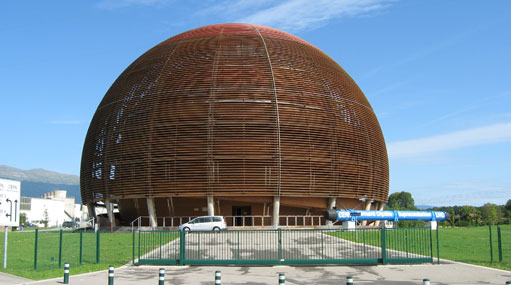
\includegraphics[height=6 cm]{cern_logo1.jpg}
	\vspace{3mm}
	\HRule 
	
	\emph{Autor:} \\
	Arthur \textsc{Oviedo}\\
    \vspace{0.5cm}
    \emph{Supervisors:} \\   

    CERN: Nikolaos \textsc{Kasioumis} \\   
    EPFL: Karl \textsc{Aberer}\\

	\vspace{0.5cm}
    % Bottom of the page
    %\emph{Remis le: 8 janvier 2010}
	%{\large \today}


\end{center}


\end{titlepage}

\newpage
\thispagestyle{empty}
\mbox{}
%\end{titlepage}

%% start the show...

\pagenumbering{roman}
\setcounter{page}{1}
\pagenumbering{arabic}

\tableofcontents

\listoffigures
\listoftables
\chapter{Introduction}



















\chapter{Theoretical Background}
\label{chapter-theoretical_background}
Information Retrieval (IR) consists of the activity of identifying relevant documents from a collection based on some input parameters.
Different models have been developed through the evolution of the field. In the subsequent sections, the most relevant models to this work are presented.

\section{Boolean Model}
The Boolean model of Information Retrieval (BIR) was the first one to be developed and is currently one of the most used in the current implementation of IR systems because of its simplicity. It is based on the mathematical concepts of Boolean Logic and Set Theory. A formalization of this framework can be stated as follows: 

Given a set of terms $T = {t_1, t_2, ... , t_n}$ which are the terms that will be indexed (In a standard search engine this can be the set of words in a language after some normalization steps), a set of documents $D = {d_1, d_2, ... , d_n} $ where $d_i \in \mathcal{P}(T) $ that the user will search for. 
A query element $q$ is a Boolean expression over the index terms and the operators $AND$ , $OR$ and $NOT$. We define the predicate $ Relevant(q, d_i) $ if a document $d_i$ satisfies the query expression $q$.
Finally the result for query over a collection of documents can now be written as $Result(q, D) = \{d | Relevant(q, d)\}$
The benefits of this model are its simplicity, both in its formalism and in its implementation. 
The main disadvantage of  BIR are the fact that all terms are given the same importance which makes it difficult to rank results. Since all results have same importance, it is difficult also to limit the number of retrieved documents and therefore the output set can be difficult to process for the final user.

One of the key data structures for an efficient implementation of this model is the inverted index where for a given term, the index stores which documents contain it. This structure is used to efficiently solve queries by only scanning document that contain at least one of the terms in the query. Scanning a document can be done by using a standard (Also called forward) index, where for a given document, the index stores the terms associated with it. Both indexes can be implemented using hash tables.

\section{Vector Space Model}
The vector space model\cite{vector_space_model} which was developed between the 1960s and 1970s alongside the SMART Information Retrieval System. In this model, documents (from a collection $D$) and queries are represented as vectors $d$ and $q$ in a vector space where each index term corresponds to a dimension. If a term $t_i$ occurs in a given query or document, its i-th  coordinate will have a non zero value. Index terms can be keywords or phrases in the context of textual search or any other type of feature that can be extracted from the elements in a given specific context.
The scoring of a document for a given query is computed as the cosine of the angle between both vectors which can be expressed as: 
$$score(d, q) = cos\theta(d, q) = \frac{d \cdot q}{\parallel d \parallel \parallel q \parallel}  = \frac{\sum_{i=1}^{n}weight(d_i, d)*weight(q_i, q)}{\sqrt{\sum_{i=1}^{n}weight^2(d_i, d)}\sqrt{\sum_{i=1}^{n}weight^2(q_i, q)}} $$

Different weighting schemes can be employed, and the most standard one is called tf-idf (Term frequency - Inverse document frequency) where terms that appear less frequently in the corpus, are assigned higher values (Intuitively the term "the" will be less useful for identifying a relevant document than the term "Shakespeare" in the context of an English word based search engine). Therefore:

$$weight(t, d) = tf(t,d) idf(t)$$

There are several variations for each of the two components. Some approaches for $tf$ include the raw frequency; Boolean frequency: $tf(t,d) = 1$ if $t$ occurs in $d$ or 0 if not; logarithmically scaled: $tf(t,d) = 	\log(frequency(t,d) +1)$
and the augmented frequency: $tf(t,d) = 0.5 + \frac{0.5*frequency(t,d)}{ \max\{frequency(t^\prime,d) | t^\prime \in d\} }$. For computing the inverse document frequency the standard approach follows $idf = \log \frac{|D|}{1+\{d \in D: t \in d \}} $

The main drawbacks of this approach reside in the assumption that the terms are independent.

\section{Probabilistic Relevance Model}
The probabilistic relevance model was developed in 1976 by Robertson and Jones\cite{probabilistic_relevance_model}. The similarity of a document $d$ to a query $q$ is given by the probability of $d$ being relevant to $q$. It assumes there is a set $R$ that is preferred to be the answer set for $q$. The model assumes that the document in $R$ are relevant to $q$ and the documents in $\bar{R}$ are not relevant. $R$ then is the set that maximizes:

$$sim(d,q) = \frac{ P(R|d)} {P(\bar{R} |d)} $$

The importance of this model is that it serves as a solid base for state of the art information retrieval models.

\section{Okapi BM25}

The Okapi BM25 ranking function is one of the current state-of-the-art models in information retrieval\cite{okapibm25}. The actual scoring function is called BM25 and Okapi refers to the first system implementing this function in the 1980s. 
Given a query $q$ as a vector of keywords $q_{1}, q_{2}, ... , q_{n}$ then the score for a document $d$ is:

$$score(d, q) = \sum_{i=1}^{n}IDF{(q_i)}*\frac{ frec(q_i, D)}{frec(q_i, D)+k_1*((1-b)+b*\frac{|D|}{avgdl})} $$
and $$IDF(q_i) = \log{\frac{N - df(q_i)+0.5}{df(q_i)+0.5}} $$

where $frec(q_i, D)$ is the number of occurrences of keyword $q_i$ in $D$, $avgdl$ is the average length (In keywords) of a document, and $k_1$ and $b$ are free parameters. Usually $k_1 = 2$ and $b \in [0, 1]$ controls how important is the length normalization, being set normally to $0.75$. $N$ is the size of the collection, $df(q_i)$ is the number of documents that contain term $q_i$ 

A further variation that takes into account structure in the form of a document containing different fields and each of them having its own length and importance (boost) can be formulated as follows, known as BM25F can be expressed as follows:


$$score(d, q) = \sum_{i=1}^{n} \frac{weigth(q_i, d)}{k+ weigth(q_i, d)} * IDF(q_i)$$
and 
$$weight(q_i, d) = \sum_{j=1}^m \frac{frec(q_i, D, field_j)*boost_j)}{((1-b_j) + b_j*\frac{|l_j|}{avgfl_j})} $$
where $m$ is the number of different fields, $boost_j$ is the relative importance for each field, $b_j$ is analogous to the $b$ constant in the BM25 group of equations, $|l_j|$ is the length of the $field_j$ and $avgfl_j$ is the average length of the $field_j$.

\section{Latent Dirichlet Allocation}

\section{Tree Edit Distance}
As it will be discussed, one of the most common formats to represent mathematical equations, MathML, is a XML based format, and whose structure represents a rooted tree. Because of this, it makes sense to consider some models to compare and analyse mathematical expressions taking into account their natural tree structure. The most natural way of addressing this, is through the well studied abstract problem of Tree Edit Distance problem, where the idea is to compute a distance between a pair of trees. It should be noted that the development of this problem is very similar to the String Edit Distance problem.
The Tree Edit Distance problem can be formulated as follows:
Let $\Sigma$ be a finite alphabet and let $\lambda \notin \Sigma$ be a special empty symbol. Finally let $\Sigma_\lambda = \Sigma \cup \lambda$. 
Given two trees $T_1$ and $T_2$ that are labelled (That is, each node $N$ in the tree has assigned a label $l(N) \in \Sigma$ ) and ordered (That is, we are provided an order between sibling nodes), we define the following operations ($l(N_1) \rightarrow l(N_2)$) where $(l(N_1),l(N_2)) \in ((\Sigma \cup \lambda)\times(\Sigma \cup \lambda)\setminus(\lambda,\lambda)) $: \\
\textbf{Relabelling:} If $l(N_1) \neq \lambda \wedge l(N_2) \neq \lambda $. We change the label of a node in the tree $T$ \\
\textbf{Deletion:} If $l(N_2) = \lambda $. The children of $N_1$ become the children of $N_1$'s parent ($N_1$ is not the root of the tree) and occupy its position in the sibling ordering. \\
\textbf{Insertion:} If $l(N_1) = \lambda $. This is the complement operation of deletion. \\

For each of this operations $\omega = (l(N_1) \rightarrow l(N_2))$, we assign a cost function $cost(\omega)$ and for a given sequence of this transformations $\Omega = (\omega_1, \omega_2, ... , \omega_n)$ we assign a cost function $cost(\Omega) = \sum_{i=1}^{i=n} {cost(\omega_i)}$ 
We also assume that $cost(\omega)$ is a distance metric. 
With the previous definition, the distance between $T_1$ and $T_2$ can be expressed now as $ dist(T_1, T_2) = min\left\{ cost(\Omega)| \Omega \text{ is a sequence of operations that transform } T_1 \text{ into } T_2 \right\} $

A recursive formulation of the problem can be defined in the following way:

\begin{align*}
dist(T,T) &= 0 \\
dist(F_1, T) &= dist(F_1 - v, T) + cost(v \rightarrow \lambda) \\
dist(T, F_2) &= dist(T, F_2 - w) + cost(\lambda \rightarrow w) \\
dist(F_1, F_2)&=\left\{
\begin{array}{ll}
dist(F_1 - v, F_2) + cost(v \rightarrow \lambda) \\
dist(F_1, F_2 - w) + cost(\lambda \rightarrow w) \\
dist(F_1(v), F_2(w)) + dist(F_1 - T_1(v), F_2 - T_2(w)) + cost(v \rightarrow w)
\end{array}
\right.
\end{align*}  
Where $F$ is a forest, $v$ and $w$ nodes from a free, $F - v$ the forest $F$ with the deletion of the node $v$, $T(v)$  the tree rooted at $v$ and $F-T(v)$ the forest obtained by removing all the nodes in $T(v)$ from $F$	

The presented set of equations give a simple way to compute the edit distance between a pair of trees, and the most known algorithms like Zhang and Shasha's\cite{zhang_shasha} whose worst time case time bound is $O(|T_1|^2|T_2|^2)$, Klein's\cite{klein} that achieves a lower bound of $O(|T_1|^2|T_2|log|T_2|)$ or Demaine's\cite{demaine}, take into advantage the fact that the recursion relies in the solution of smaller sub-problems, so by carefully choosing which of this sub-problems to solve.


\thispagestyle{empty}




\chapter{Technical Considerations}
\label{chapter-technical_considerations}
In the previos chapter we presented different abstract models which can be suitable in the building of a math based search system.
In this section, we present different aspects that need to be considered when mapping from these theoretical models to a concrete implementation.

\section{Digital Representations of Mathematics}
When building any kind of information retrieval system, selecting the right representations of the data can affect the type of algorithms that one can use, the amount of storage, the quality of the data among other factors. Mathematical content is not an exception, and there are available different formats to encode a mathematical expression. One of the most common ways to represent mathematics in scientific documents, which suits CDS's domain, is \LaTeX. 

Another  important standard for the representation of mathematics is MathML, which was first proposed by the World Wide Web Consortium in 1998 as the recommended language to be used in web documents. One of the advantages of MathML over LaTeX, is the fact that it is an application of XML, which makes it very easy process algorithmically. There two different variations of MathML, presentation and content. The first one is oriented to the visual representation of the expression and the second one is more oriented to the semantics of the expression. Its main component is the <apply> tag which represents the function application . 

OpenMath is yet another markup language to represent mathematics and can be used to compliment presentation MathML to add more semantic information. It is mainly used now for defining mathematical concepts into standard content dictionaries which can be imported. MathML is compatible with this dictionaries.

Table \ref{math_languages} presents a comparison on how different languages can express the quadratic equation $x = \frac{-b \pm \sqrt{b^2 - 4ac}}{2a} $


\begin{longtable}{|>{\centering\arraybackslash}m{3.5cm}|>
{\centering\arraybackslash}m{3cm}|>
{\centering\arraybackslash}m{3cm}|>
{\centering\arraybackslash}m{5cm}|
}
\hline 
\textbf{\LaTeX} & 
\textbf{Presentation MathML} & 
\textbf{Content MathML + Presentation Markups} & 
\textbf{OpenMath}  \\ \hline

\scriptsize{\lstinline|$x = \frac{-b \pm \sqrt{b^2 - 4ac}}{2a} $|}
& \scriptsize{\codefont <math display="block"> <mrow>   <mi>x</mi>  <mo>=</mo>  <mfrac> <mrow> <mo>-</mo> <mi>b</mi> <mo>
{\unicodefont \char"00B1} </mo> <msqrt> <msup> <mi>b</mi> <mn>2</mn> </msup> <mo>-</mo> <mn>4</mn> <mo></mo> <mi>a</mi> <mo></mo> <mi>c</mi> </msqrt> </mrow> <mrow> <mn>2</mn> <mo></mo> <mi>a</mi> </mrow> </mfrac> </mrow> </math>}
&
\scriptsize{\codefont <math> <apply> <eq/> <ci>x</ci> <csymbol> <mfrac> <apply> <minus/> <mi>b</mi> {\unicodefont \char"00B1} <mroot> <apply> <minus/> <csymbol> <msup> <mi>b</mi> <mn>2</mn> </msup> </csymbol> <csymbol> <mn>4</mn> <mo>\&times;</mo> <mi>a</mi> <mo>\&times;</mo> <mi>c</mi> </csymbol> </apply> <mrow></mrow> </mroot> </apply> <apply> <times/> <cn>2</cn> <ci>a</ci> </apply> </mfrac> </csymbol> </apply> </math> } 
&
\scriptsize{\codefont 
<OMOBJ> <OMA> <OMS cd = "relation1" name="eq"/> <OMV name="x"/>
    <OMA> <OMS cd="arith1" name="divide"/> <OMA> <OMS cd = "arith1" name="minus"/><OMA> <OMS cd = "arith1" name="times"/>
          <OMA> <OMS cd = "arith1" name="times"/> <OMV name="b"/> <OMV name="+ALE-"/> </OMA> <OMA> <OMS cd="arith1" name="root"/> <OMA> <OMS cd = "arith1" name="minus"/> <OMA> <OMS cd="arith1" name="power"/> <OMV name="b"/> <OMI>2</OMI> </OMA> <OMA> <OMS cd = "arith1" name="times"/> <OMA> <OMS cd = "arith1" name="times"/> <OMI>4</OMI> <OMV name="a"/> </OMA> <OMV name="c"/> </OMA> </OMA> <OMA> <OMI> 2 </OMI> </OMA> </OMA> </OMA> <OMA> <OMS cd = "arith1" name="times"/> <OMI>2</OMI> <OMV name="a"/> </OMA> </OMA> </OMA> </OMOBJ>}
\\
\hline

\caption{Comparison of the different languages for expressing mathematical content} 
\label{math_languages}
\end{longtable}

\LaTeX allows the most compact representations of the equations and it is the closest language to the community. However, its processing is not straightforward because a given equation can include multiple commands from different packages. Also there are several ways to represent the same set of symbols, either using its Unicode code-point or through embedded commands. Another difficulty are custom commands that users can define in the preamble of the document. In overall, the interpretation and processing of a mathematical expression in this language would require writing a complete compiler which is not the purpose of this work. MathML offers a better compromise between the length of the representation and the easiness to be processed.

\section{Math Extraction Tools}
One of the main steps in any information retrieval task is the extraction of the searchable content from the collection of documents. At CDS the most common storage format for publications is PDF. A big part of the harvested documents in CDS comes from the ArXiv pre-prints service and from here, the source code (\LaTeX) of the submissions is available for download. Smaller portions of other documents are stored in other formats like Microsoft Word, OpenOffice Documents.
In practice, the main options from where to do the extraction from, are PDFs and \LaTeX  files. Also taking into account the previous discussion on the available format for representing mathematics, we focused our attention in tools that output MathML.  \\
A conscious exploration of available software for extracting mathematical content from this two types of documents allowed us to identify different tools with different approaches. 
\LaTeX  files are easier to process and all of the tools implement their own compiler that XML + MathML outputs instead of the typical. Since the original math equation is provided in the document, there is relatively little ambiguity in the equation, and the major issues that the systems struggle with is in the coverage of all the possible commands and packages that are available. \\
For extracting equations from PDF files, the process turns into an Optical Character Recognition (OCR). The reconstruction of the equation has to infer the mathematical structure based on physical positioning and size of the symbols, the length of the lines and so on.

Table \ref{math_extraction_tools} presents the main features of the reviewed software. 

\begin{longtable}{|>{\centering\arraybackslash}
m{2.93cm}|>{\centering\arraybackslash}
m{1.8cm}|>{\centering\arraybackslash}
m{1.6cm}|>{\centering\arraybackslash}
m{1.9cm}|>{\centering\arraybackslash}
m{1.6cm}|>{\centering\arraybackslash}
m{1.8cm}|>{\centering\arraybackslash}
m{1.4cm}|
}
\hline 
\small{\textbf{Software}} & \small{\textbf{Type}} & \small{\textbf{Tested version}} & \small{\textbf{Input Format(s)}} & \small{\textbf{Output Format(s)}} & \small{\textbf{Licence Type}} & \small{\textbf{Latest Update}}  \\
\hline
\small{LaTeXML}\cite{latexml} & \small{Standalone Executable} & \small{0.7.9alpha} & \small{\LaTeX} & \small{XML + MathML} & \small{Open Source} & \small{13 Feb 2014}  \\
\hline
\small{TeX4ht}\cite{tex4ht2} & \small{Standalone Executable} & \small{ 2009-01-31-07} & \small{\LaTeX} & \small{XML + MathML} & \small{ Open Source} & \small{11 Jun 2009}  \\
\hline
\small{SnuggleTex}\cite{snuggletex} & \small{Java Library} & \small{1.2.2} & \small{\LaTeX (Small fragments)} & \small{MathML} & \small{Open Source} & \small{24 May 2010}  \\
\hline
\small{LaTeXmathML}\cite{latexmathml} & \small{Javascript Library} & \small{30-October-2007} & \small{\LaTeX} & \small{XML + MathML} & \small{Open Source} & \small{30 Oct 2007}  \\
\hline
\small{Maxtract}\cite{maxtract1}\cite{maxtract2} & \small{Standalone Executable} & \small{v.1752} & \small{PDF} & \small{\LaTeX / Annotated PDF} & \small{Free to download} & \small{15 Nov 2012}  \\
\hline
\small{InftyReader}\cite{infty1}\cite{infty2} & \small{Standalone Executable (On Windows)} & \small{2.9.6.2} & \small{PDF, TIFF, BMP, GIF, PNG} & \small{\LaTeX, XML + MathML} & \small{Commercial} & \small{22 Dec 2013}  \\

\hline
\caption{Comparison of available Mathematical extraction tools}
\label{math_extraction_tools}
\end{longtable}

For extraction from \LaTeX  files we concluded that the best option is LaTeXML. The tool is still in current development and has lot of support from the academic community. The performance on a small dataset also showed that the results are consistently better than from the other tools. A more thorough test\cite{latexcomparison} also confirms that LaTeXML provides the best results. For PDF files, the trial version of InftyReader worked very well giving better results and processing successfully more files than Maxtract. As said previously, a big portion of the documents stored in CDS, come from pre-printing services like ArXiV were fortunately the source code of an article is available and because of this reason, our base set for this work will consist on extracting equations from \LaTeX files. For licensing reasons, for this project we will not integrate our system with InftyReader for the moment and will proceed with LaTeXML as our extraction tool.



\section{Computer Algebra Systems}
Computer Algebra Systems (CASs) are software packages that allow performing symbolic transformations on mathematical objects. They allow to manipulate, simplify and analyse mathematical equations and offer interesting functionalities for a mathematical based search engine. The most important functionalities that we are looking for in such system are simplification and normalization of mathematical expressions and pattern matching. As discussed previously, the language for representing expressions will be MathML, so we also require that such system is able to import this format. Finally, we are also interested in integrating these functionalities in a bigger system, so integration trough APIs was also considered.


\begin{longtable}{|>
{\centering\arraybackslash}m{2cm}|>
{\centering\arraybackslash}m{2.1cm}|>
{\centering\arraybackslash}m{1.9cm}|>
{\centering\arraybackslash}m{1.55cm}|>
{\centering\arraybackslash}m{1.83cm}|>
{\centering\arraybackslash}m{1.95cm}|
}
\hline 
\textbf{\small{CAS}} & 
\textbf{\small{Imports MathML}} & 
\textbf{\small{Expression normalization}} & 
\textbf{\small{Pattern Matching}}  &
\textbf{\small{License Type}}  &
\textbf{\small{Supported APIs}}
\\
\hline
\small{Maple} &  \small{Yes} & \small{Yes} & \small{Yes} & \small{Commercial} & \small{C, Java, VB} \\ \hline
\small{MatLab (Symbolic Math Toolbox)} & \small{Experimental} & \small{Yes} & \small{Yes} & \small{Commercial} & \small{C/C++, Fortran} \\ \hline
\small{Mathematica} & \small{Yes} & \small{Yes} & \small{Yes} & \small{Commercial} & \small{C, Java, .NET} \\ \hline 
\small{Maxima} &  \small{Experimental} & \small{Yes} & \small{Yes} & \small{Open Source} & \small{C++, Java (External Project)} \\ \hline
\small{SymPy} & \small{No} & \small{Yes} & \small{Yes} & \small{Open Source} & \small{Python} \\ \hline

\caption{Comparison of main CAS}
\label{CAS_comparison}
\end{longtable}

Table \ref{CAS_comparison} presents a comparison of the desired features in the main CASs. The systems that better fit our requirements are Maple and Mathematica. For licensing reasons, we will continue our project using Mathematica.





\chapter{Related Work}
\label{chap-related_work}
\section{Status of Mathematical Information Retrieval}
Even though Information Retrieval has been a research field from around the 1950s where the first metrics for such systems were developed and in the 1960s where SMART (System for Mechanical Analysis and Retrieval of Text), the first computer based system was developed; only in the last couple years focus have been put into adapting the same techniques to mathematical content. 

The Mathematics Information Retrieval Workshop\cite{mir_workshop} held in the context of the Conference of Intelligent Computer Mathematics in July 2012, was the first official event in the area of MIR. Here, a small competition was held to evaluate different systems and approaches.

The NII\cite{nii} (National Institute of Informatics) is a Japanese research institute that hosts the project named NTCIR (NII Testbeds and Community for Information access Research) which aims to build evaluation frameworks for specific sub-fields of information retrieval. On 2013, in the context of the 10th NTCIR conference, it hosted the NTCIR-10 Math Task \cite{math_task} which was the first collaborative effort to evaluate different systems. The Math task was focused on two different subtasks: Math retrieval (Identifying relevant document based on given mathematical expressions and/or keywords) and Math understanding where the idea was to extract natural language information of a mathematical expression in a document. Currently submissions are open for the NTCIR-11 Math Task 2 which will be held on December 2014.

\section{Mathematical based search projects}

\subsection{MIaS}
MIaS\cite{mias_1} (Math Indexer and Searcher), currently, is one of the flagship projects in the indexing and searching of mathematical content. As most of the other projects, it processes documents in MathML format. It allows the user to include in the queries mathematical expressions and textual content. During indexing time, equations are transformed following a set of heuristics that include:
\begin{itemize}
  \item Ordering of elements: Taking into account commutativity of certain operators (Addition, multiplication), elements are ordered such that $3 + a$ would be converted into $a + 3$ (Since the <mi> tag comes first than the <mn> tag)
  \item Unification of variables: This process takes into the account the structure of the equations in despite of the naming of the variables. Expressions like $a+b^a$ and $x+y^x$ would be converted into an expressions of the form $id_1 + id_2^{id_1}$ which would match.
  \item Unification of constants: This step consists of replacing all occurrences of constants (<mn> tags) by a const symbol. 
\end{itemize}
The extracted tokens from a given equation consist of all its valid sub-expressions. The original expression is given a weight value of 1, and following sub-expressions are given smaller weights depending on how general or specific they are.  
The system, also as most of the current projects, is developed by using the Apache Lucene framework. The system adapts the default scoring equation such that the given weight is taken into account.  
Publicly available instances of the system can be found at: \url{http://aura.fi.muni.cz:8085/webmias/ps?n=-1} running on the MREC\cite{mrec} dataset and  \url{ http://aura.fi.muni.cz:8085/webmias-ntcir/} (Running on the NTCIR dataset)

\subsection{EgoMath}
EgoMath\cite{egomath1} and its new version EgoMath$^2$\cite{egomath2}, is a system oriented to index the mathematical content from the Wikipedia.org database. The processing steps before indexing are similar to the ones in MIaS (Rearranging of symbols, unification of constants). The extraction process started from a complete dump of the Wikipedia database and filtering only the math articles, which are identified by the ”<math>" tag. This consists on around thirty thousand articles, from which 240.000 equations were identified. The processing step includes translating the equation from LaTeX into MathML format and then indexing both representation.
Some additional effort is done into splitting large mathematical blocks like tables into single mathematical expressions. At the start of this work, EgoMath was publicly available at \url{http://egomath.projekty.ms.mff.cuni.cz/}, however at this moment the system seems to be unavailable.

\subsection{DLMFSearch}
The Digital Library for Mathematical Funtions \cite{dlmf} is a project launched by the National Institute of Standards and Technology, in 2010, as an online version of the  Handbook of Mathematical Functions with Formulas, Graphs and Mathematical Tables\cite{handbook}. DLMF's main goal is to compile the mathematical knowledge in the form of equations, functions, tables and make this information useful for researchers and public in general. The system contains a search functionality that allows to input a combination of full text and \LaTeX snippets. The system tries to perform an exact match, and if no results are found, it relaxes the query. DLMF also perfoms some normalization of the equation and some cleaning of some characters, but no further details are provided. The content indexed by this project is highly curated, which differentiates it from the other projects. In the report published in 2013 \cite{dlmf2}, it is reported to have indexed around 38000 equations. This project is publicly available at \url{http://dlmf.nist.gov/}

\subsection{MathWebSearch}
MathWebSearch\cite{mathwebsearch} (Currently on its 0.5 version) is a open-source search engine for mathematical equations. While most of the documentation relates on the architecture of the system and how they address scalability; the indexing technique is also very interesting. The system implements and idea proposed by Peter Graf in \cite{substitution_tree_indexing} called substitution tree indexing. This idea can be viewed as a generalization of the variable and constant unification. It represents the equations as a tree an recursively generalizes each sub-expression. A public available instance of the system is available at \url{http://search.mathweb.org/tema/} which runs on the Zentralblatt Math database\cite{zb}.


\subsection{LaTEXSearch}
LaTEXSearch \url{http://latexsearch.com/} is a system developed by the scientific publisher Springer that allows to search over a database of around eight million latex snippets extracted from their publications. The system, unfortunately, is proprietary and no details are provided about the internals of the system.

\subsection{WikiMirs}
WikiMirs\cite{wikimirs} is a system that, as EgoMath, allows to find relevant Wikipedia entries by providing mathematical expression in \LaTeX. It combines the information about the semantic tree with the layout tree of a given expression and uses a similar approach to index different generalization levels.

Other systems that provide similar search functionalities are \url{Uniquation} and \url{http://www.symbolab.com/}, however detailed information about the systems are not provided. Finally Wolfram Alpha\cite{wolframalpha} is a very powerful tool that allows to find information about lots of mathematical concepts and a wide variety of other objects (Even Pokemon).



\chapter{MASE(CDS)}
\label{chapter-cern_math_explorer}
In this chapter we present our solution called MASE(CDS), Math Aware Search Engine (For CDS). We present the key points of our system, and how they are related to previous built systems.

\section{Features Extraction}
Our main goal is to develop a system that compliments the already available search capabilities in Invenio and in particular the CDS instance. Our system was developed on top of the  the Apache Solr/Lucene framework. CDS already uses Solr as a search engine layer, so developing MASE using this technology supposed a reasonable choice. One of the main steps while building an IR tool, is understanding the data and what kind of features can be extracted from it: If the system is based on text, then tasks as stemming, handling of synonyms, misspelling and so on, such be taken into consideration; if the system being developed is based on images, then examples of features can be histograms of colors, geometrical features and so on. During the literature review, we discovered that most of the projects handled the notational aspects of the expressions, that is, the real naming of the terms in a given equation and each project developed its own set of heuristics to handle the structural component. 


\subsection{Notational Features}
Notational features correspond to the elements that relate to the actual naming of the variables, constants and numeric quantities found in an equation. Here we extract tokens that represent single leaf nodes (E.g. <mi>, <mn>, <mo> tags), and simple constructs like subscript and superscript elements, fractions, roots.
We also extract bi-grams and tri-grams as analogue to that is done for text indexing in current systems.

After examining a set of relevant documents from our dataset, we identified some heuristics that could be applied to improve the recall of our system:



\subsubsection{Unicode Normalizing} 
The first issue we discovered is that because of the big wide of different characters to represent the possible mathematical symbols, there is need for an automatic way to match different possible variations of a single character. An example of this situation is specification of an natural number, sometimes denoted by the letter N. In this case, at least three different common representations were identified: $ N = 1 $ (Using character with unicode code point 0x004e), $\mathcal{N} = 1$ (0xd835 0xdc41 or in latex expressed as \lstinline|\mathcal{N}|) and $\mathbb{N} = 1$ (0x2115 or in latex expressed as \lstinline|\mathbb{N}|). \\
  For addressing this situation, we rely on the Unicode equivalence framework. In the unicode specification, sometimes the same character have two or more different code-points because of backwards compatibility with other encoding standards or because the same character has different essential meanings. Another group of equal characters with different code-points are pre-combined characters such as the Latin letter \~{N} which has Unicode point 0x00D1 and also is the sequence of code-points  0x004E (Latin letter N) and 0x0303 (the combining character tilde). Taking this sample into account, Unicode defines the character composition and decomposition operations as replacing the decomposed representation with the pre-composed one and vice-versa. Finally, Unicode defines two types of equivalences between characters: Canonical and compatible. Canonical equivalent characters are assumed to have the same appearance and meaning. Compatible ones are allowed to have slightly different graphical representations but the same meaning in some contexts. One example of compatible equivalent characters is the Roman number 12 {\unicodefontⅫ} with code-point 0x216b and the sequence of characters XII with codepoints 0x0058 0x0049 0x0049. Taking into account the composition or decomposition of characters and the canonical or compatible equivalences, Unicode specifies 4 different forms of a given character:
  \begin{itemize}
  \item NFD: Normalization Form Canonical Decomposition
  \item NFC: Normalization Form Canonical Composition
  \item NFKD: Normalization Form Compatibility Decomposition
  \item NFKC: Normalization Form Compatibility Composition
  \end{itemize}
  
Table \ref{unicode_characters} presents a small list of troubling characters classes that were identified in our datasets.

\begin{longtable}{|m{4cm}|>{\centering\arraybackslash}m{2.15cm}|>{\centering\arraybackslash}m{1.65cm}|>{\centering\arraybackslash}m{1.65cm}|>{\centering\arraybackslash}m{1.65cm}|>{\centering\arraybackslash}m{1.65cm}|}
\hline 
\textbf{Character Name} & \textbf{Visual Rendering} & \textbf{NFC} & \textbf{NFD} & \textbf{NFKC} & \textbf{NFKD} \\ 
\hline 
LATIN CAPITAL LETTER A & A & 0x41 & 0x41 & 0x41 & 0x41 \\ 
\hline 
LATIN CAPITAL LETTER A WITH MACRON & \={A} & 0x100 & 0x41 0x304 & 0x100 & 0x41 0x304 \\
\hline 
LATIN CAPITAL LETTER A WITH RING ABOVE & \r{A} & 0xc5 & 0x41 0x30a & 0xc5 & 0x41 0x30a \\
\hline 
ANGSTROM SIGN (0x212b) &	\r{A} &	0xc5 &	0x41 0x30a &	0xc5 &	0x41 0x30a \\
\hline
LATIN CAPITAL LIGATURE IJ &	IJ &	0x132 &	0x132 &	0x49(I) 0x4a(J) &	0x49 0x4a \\
\hline
CYRILLIC CAPITAL LIGATURE A IE & {\unicodefont Ӕ} &	0x4d4 &	0x4d4 &	0x4d4 &	0x4d4 \\
\hline
LATIN CAPITAL LETTER AE	& {\unicodefont Ӕ}	& 0xc6	& 0xc6	& 0xc6	& 0xc6 \\
\hline
DOUBLE-STRUCK CAPITAL N	& {\unicodefont ℕ}	& 0x2115 & 0x2115 & 0x2115 & 0x4e \\
\hline
LATIN CAPITAL LETTER N	& N & 0x4e	& 0x4e & 	0x4e	& 0x4e \\
\hline 
MATHEMATICAL ITALIC CAPITAL N & $\mathcal{N}$	& 0xd835  0xdc41 &	0xd835  0xdc41 &	0x4e	 & 0x4e \\
\hline 
ROMAN NUMERAL TWELVE	& {\unicodefont Ⅻ}	&0x216b &	0x216b	& 0x58 0x49 0x49 &	0x58 0x49 0x49 \\
\hline
LATIN CAPITAL LETTER X - LATIN CAPITAL LETTER I - LATIN CAPITAL LETTER I &	XII &	0x58 0x49 0x49 &	0x58 0x49 0x49&	0x58(X) 0x49(I) 0x49(I) &	0x58 0x49 0x49 \\
\hline
VULGAR FRACTION ONE QUARTER	& \char"00BC &	0xbc &	0xbc &	0x31(1) 0x2044(/) 0x34(4) &	0x31 0x2044 0x34 \\
\hline
DIGIT ONE - SOLIDUS - DIGIT 4 &	1⁄4 &	0x31  0x2f 0x34 &	0x31 0x2f 0x34	& 0x31 0x2f 0x34 &	0x31 0x2f 0x34\\
\hline
DIGIT ONE - SOLIDUS - DIGIT 4 &	1⁄4 &	0x31  0x2f 0x34 &	0x31 0x2f 0x34	& 0x31 0x2f 0x34 &	0x31 0x2f 0x34\\
\hline
DIGIT ONE - FRACTION SLASH - DIGIT 4 & 1⁄4 &	0x31 0x2044 0x34 &	0x31 0x2044 0x34 &	0x31 0x2044 0x34 &	0x31 0x2044 0x34 \\
\hline
THERE EXISTS	& {\unicodefont ∃}&	0x2203 &	0x2203 &	0x2203 &	0x2203 \\
\hline
THERE DOES NOT EXIST	& {\unicodefont ∄} & 	0x2204	& 0x2203 0x338& 	0x2204 &	0x2203 0x338\\
\hline
LATIN CAPITAL LETTER OPEN E	& {\unicodefont Ɛ} &	0x190 &	0x190 &	0x190 &	0x190 \\
\hline
EULER CONSTANT	& {\unicodefont ℇ} & 0x2107 & 0x2107 & 0x190 & 0x190 \\
\hline
PLANCK CONSTANT	& {\unicodefont ℎ} &	0x210e &	0x210e &	0x68 &	0x68 \\
\hline
LATIN SMALL LETTER H &	h &	0x68 &	0x68 &	0x68 &	0x68 \\
\hline
PLANCK CONSTANT OVER TWO PI	& {\unicodefont ℏ} &	0x210f &	0x210f	& 0x127 &	0x127 \\
\hline
LATIN SMALL LETTER H WITH STROKE & ħ &	0x127	& 0x127	& 0x127	& 0x127 \\
\hline
GREEK CAPITAL LETTER OMEGA	& Ω &	0x3a9 &	0x3a9 &	0x3a9 &	0x3a9 \\
\hline
OHM SIGN & Ω &	0x2126 &	0x2126 &	0x3a9 &	0x3a9 \\
\hline
INTEGRAL & {\unicodefont ∫} &	0x222b &	0x222b &	0x222b &	0x222b \\
\hline
DOUBLE INTEGRAL	& {\unicodefont ∬} & 	0x222c &	0x222c &	0x222b 0x222b &	0x222b 0x222b \\
\hline
CONTOUR INTEGRAL	& {\unicodefont ∮} &	0x222e	 &0x222e &	0x222e &	0x222e \\
\hline
\caption{Characters with similar glyphs and/or semantics}
\label{unicode_characters}
\end{longtable}


Since our goal is to match as much as possible similar characters, our system employs the NFKD representation of a character. For a given token, we test whether if it is already equal to its NFKD. If not, for all the characters that are not combining nor control characters, we add the token into the same position as the original one.
For example, given the token <mi>\r{A}</mi>, this will lead to the sequence <mi>\r{A}</mi><mi>A</mi> and the token <mi>{\unicodefontⅫ}</mi> will produce <mi>{\unicodefontⅫ}</mi><mi>X</mi><mi>I</mi><mi>I</mi>.

\subsubsection{Synonym Expansion}
Even though the Unicode normalization step work for a big part of the cases presented in table \ref{unicode_characters}, there are still some groups of characters which would not be matched (Even partially), such as some types of integrals. For addressing these groups, a precomputed table was created for some general groups of characters which have some similar meaning. For each token that belongs to some of this predefined groups, a second token is created identifying the group.
For example the token <mo>{\unicodefont ∮}</mo> is expanded into <mo>{\unicodefont ∮}</mo><mo>INTEGRALS</mo>, similarly the token token <mo>{\unicodefont ∫}</mo> is expanded into <mo>{\unicodefont ∫}</mo><mo>INTEGRALS</mo> and then both will have a partial match in the INTEGRALS token. 
Unicode specification does not define a strict rule to group similar characters based on their semantics. For general operators, we used the grouping provided by Xah Lee in his website\cite{math_groups}.

\subsubsection{Numeric Approximation} 
Some equations relate specific numeric quantities. While most of the previously explorer systems, handled <mn> tags by only representing them as a constant identifier, this approach is not suitable. A lot of articles in CDS relate to specific experiments under certain conditions, and require a high level of precision in the measurements. However, different experiments of the same phenomenon, can result in different measurements and we wanted to include this variability in our system. To handle this, when a token with a certain numeric quantity is discovered, we apply iterative rounding and index all the different approximations in the same position as the original element. For example the token <mn>2.0135</mn> will produce the following sequence of tokens: <mn>2.0135</mn><mn>2.014</mn><mn>2.01</mn><mn>2.0</mn>. 


\subsection{Structural Features}


\subsubsection{Algebraic structures}
The first set of structures consist on purely algebraic relationships between the expressions.
Inspired by predefined integral tables for different kinds of expressions, we decided to extract from a given equation, whether it has the occurrence of these kind of patterns.
An example of this type of structures would be: $X\textunderscore*(X\textunderscore + A\textunderscore)$ where $X\textunderscore$ and $A\textunderscore$ can be any type of expression. Sample equations matching this pattern can be $C (C+1)$ or $\frac{(\sin{\theta}\cos{\theta})^2}{2a} (\frac{(\sin{\theta}\cos{\theta})^2}{2a} + \tan{\frac{\theta+\phi}{2}})$. This structural analysis of equations is more powerful than the unification of variables and constants proposed in previously discussed projects because these patterns, as shown in the second example, can match an arbitrary complex expression. The drawback of our solution is the need to manually select representative and useful patterns. This selection was done based on standard based tables of integrals similar to the ones that Computational Algebraic Systems employ to compute them.

\subsubsection{Non-formal mathematical variations}
This set of structures represent common operations that cat appear in a given expression, but its identification is based on notation factors. A simple example of this can be the matrix decomposition $A = VDV^{-1}$ where the actual name of the variables $A$ and $V$ is not meaningful but the real importance is the fact that a given variable appears alongside its inverse in a matrix multiplication form. We would like to assign a partial match to any other kind of this decomposition say $B = MRM^{-1}$. these types of structures live in-between the notational and structural categories but, as it will be discussed, we identify them using Mathematica and encompass them as structural features.

\subsubsection{Specific domain structures}
Additionally, we identified patterns that are relevant and frequent in specific domains of the high energy physics.


\subsection{Development with Lucene/Solr}
This section explains how the described features were implemented in the \verb|Apache Solr/Lucene| framework.
\subsection{Integration with Mathematica}
This section describes some aspects that should be had to be considered while implementing the integration with the Mathematica CAS. Our system uses the provided \verb|JLink| library to create a connection with the underlying process \verb|MathKernel|. The main class for communicating java code and \verb|Mathematica| is \verb|KernelLink| and the main used method was \verb|evaluateToOutputForm(String expr, int pageWidth)| where \verb|expr| is the expression to be evaluated and \verb|pageWidth| affects the formatting of the result.

\subsubsection{Pattern Extraction}

\subsubsection{Recursive interpretation}

\subsubsection{Error handling}
Sometimes, after certain time, the connection between \verb|KernelLink| and \verb|Mathematica| will be lost launch an exception and following invocations would fails as well.
Also, re-instantiating a KernelLink will yield an Exception. For this scenario, killing the associated processes to Mathematica was necessary:

\begin{verbatim}
killall -s 9 Mathematica
killall -s 9 MathKernel
\end{verbatim} 

or 

\begin{verbatim}
taskkill /im Mathematica.exe
taskkill /im MathKernel.exe
\end{verbatim} 

Depending on the OS the system is running on.

With this, the next creation of a new KernelLink works properly and the subsequent invocations work as expected.

\subsubsection{Timeout Handling}
Unfortunately, checking the quality of a LaTeX document is a difficult job and users have a lot of freedom in the way they write their document since the only visible result is the rendered version. 
One example we found during our work is the following TeX snippet:
\begin{verbatim}
	"\ \varphi\ are\ shown,\ as\ well\ as\ the\ weight\ and\ tension"
\end{verbatim}
A human can easily identify that this corresponds to text and that should be inserted into a proper "mbox" or "text" tag. In this case, the snippet produced the following MathML code
\begin{verbatim}
<math><mrow><mi>φ</mi><mo></mo><mrow><mi>a</mi><mo></mo><mi>r</mi>   
<mo></mo><mi>e</mi></mrow><mo></mo><mrow><mi>s</mi><mo></mo>
<mi>h</mi><mo></mo><mi>o</mi><mo></mo><mi>w</mi><mo></mo><mi>n</mi>
</mrow><mo>,</mo><mrow><mi>a</mi><mo></mo><mi>s</mi></mrow><mo></mo>
<mrow><mi>w</mi><mo></mo><mi>e</mi><mo></mo><mi>l</mi><mo></mo>
<mi>l</mi></mrow><mo></mo><mrow><mi>a</mi><mo></mo><mi>s</mi>
</mrow><mo></mo><mrow><mi>t</mi><mo></mo><mi>h</mi><mo></mo>
<mi>e</mi></mrow><mo></mo><mrow><mi>w</mi><mo></mo><mi>e</mi><mo>
</mo><mi>i</mi><mo></mo><mi>g</mi><mo></mo><mi>h</mi><mo></mo>
<mi>t</mi></mrow><mo></mo><mrow><mi>a</mi><mo></mo><mi>n</mi><mo>
</mo><mi>d</mi></mrow><mo></mo><mrow><mi>t</mi><mo></mo><mi>e</mi>
<mo></mo><mi>n</mi><mo></mo><mi>s</mi><mo></mo><mi>i</mi>
<mo></mo><mi>o</mi><mo></mo><mi>n</mi></mrow></mrow></math>
\end{verbatim}

Mathematica took around 10 minutes to interpret it.
In the ideal case we would be able to identify the malformed expressions and pass to Mathematica only well-formed equations to be processed but as this simple example shows, that is a very challenging task and may require more work.
As a remedial situation, we used a fixed timeout to stop the processing of a given expression.

\subsection{Integration with CDS}

\chapter{Evaluation}
...

\section{Dataset}
Our dataset consists on 12234 latex documents fetched from ArXiV. This documents correspond to the latest records harvested for CDS. The documents were processed using LateXML as described in the extraction process. From the given dataset, the simpler equations were filtered out (The ones containing one or two elements).


\section{Setup}

The machine used for experiments has a Intel Core i7 processor running at 3.4Ghz with 4 cores. The available RAM is 8Gb, and the Java Virtual Machine used for running Solr was run with the $-Xms2G -Xmx5G$ parameters. The complete specifications of the used software is presented in table \ref{sw_used}

\begin{longtable}{|m{2cm}|>
{\centering\arraybackslash}m{4cm}|>
{\centering\arraybackslash}m{4cm}|
}
\hline 
\textbf{Software} & 
\textbf{Version} 
\\
\hline
Operative System & Linux Mint 16 Petra (Ubuntu based) \\ \hline
Linux Kernel & 3.11.0-15 \\ \hline
Java Virtual Machine & 1.7.0-45 \\ \hline
Apache Solr & 4.6 \\ \hline
Python & 2.7.5+ \\ \hline
\caption{Software used during evaluations}
\label{sw_used}
\end{longtable}

\section{Results quality}
In this section we are interested in evaluating the quality of the results provided by our system.
The type of queries that MASE was designed for, are typical equations that can be found in a scientific publication. 
Out main user case is that a user of CDS is interested in finding documents inside the collection whose equations are related to the one that is provided.

\subsection{Equations}
The evaluated queries were provided by physics experts working at CERN from their own research topics. The queries were provided in \LaTeX format as the users used them in their own publications.
Table \ref{equations_table} presents the set of queries that were evaluated, and a simple explanation about it. 


\begin{longtable}{|m{0.75cm}|>
{\centering\arraybackslash}m{2.7cm}|>
{\centering\arraybackslash}m{6.5cm}|>
{\centering\arraybackslash}m{5cm}|
}
\hline 
\textbf{Id} & 
\textbf{Description} &
\textbf{MathML code} &
\textbf{Visual Form}


\\
\hline
Eq1 & \scriptsize{ Time-independent Schr\char"00F6dinger equation} & \scriptsize {\codefont <math><mfenced close=")" open="("> <mrow> <mo>-</mo> <mfrac> <msup> <mi>ℏ</mi> <mn>2</mn> </msup> <mrow> <mn>2</mn> <msub> <mi>m</mi> <mi>e</mi> </msub> </mrow> </mfrac> <msup> <mo>$\nabla$</mo> <mn>2</mn> </msup> <mo>+</mo> <mi>V</mi> <mfenced close=")" open="("> <mi>r</mi> </mfenced> </mrow> </mfenced> <mi>ψ</mi> <mfenced close=")" open="("> <mi>r</mi> </mfenced> <mo>=</mo> <mi>E</mi> <mi>ψ</mi> <mfenced close=")" open="("> <mi>r</mi> </mfenced> </math>} & \scriptsize{ $\left (-\frac{\hbar^{2}}{2m_e}\nabla^{2} + V(\mathbf{r})\right )\psi(\mathbf{r}) = E\psi(\mathbf{r})$ }\\ \hline

Eq2 & \scriptsize{Atomic mass in terms of number of proton and number of neutrons} & \scriptsize {\codefont <math> <mi>A</mi> <mo>=</mo> <mi>Z</mi> <mo>+</mo> <mi>N</mi> </math>} & \scriptsize{$A = Z + N$} \\ \hline

Eq3 & \scriptsize{Radiation flux in term of the initial intensity, the absorption coefficient and the thickness of a substance} & \scriptsize {\codefont <math> <mi>I</mi> <mo>=</mo> <msub> <mi>I</mi> <mn>0</mn> </msub><msup> <mi>e</mi> <mrow> <mo>-</mo> <mi>μ</mi> <mi>x</mi> </mrow> </msup> </math>
} & \scriptsize{$I = I_0e^{-\mu x}$ } \\ \hline

Eq4 & \scriptsize{Higgs Boson decaying process into $W^+$ and $W^-$ bosons. This is not exactly a mathematical equation, but a physical process. However it is also expressed in LaTeX and to high energy physics experts, it makes sense to search them.} & \scriptsize {\codefont <math> <mi>H</mi> <mo>→</mo> <msup> <mi>W</mi> <mo>+</mo> </msup> <msup> <mi>W</mi> <mo>-</mo> </msup> </math>} & \scriptsize{$H\rightarrow W^+W^-$ } \\ \hline

Eq5 & \scriptsize{Einstein Field equation} & \scriptsize {\codefont <math><msub><mi>G</mi><mrow><mi>μ</mi><mi>ν</mi></mrow></msub><mo>=</mo><msub><mi>R</mi><mrow><mi>μ</mi><mi>ν</mi></mrow></msub><mo>-</mo><mfrac><mn>1</mn><mn>2</mn></mfrac><mi>R</mi><msub><mi>g</mi><mrow><mi>μ</mi><mi>ν</mi></mrow></msub><mo>=</mo><mfrac><mrow><mn>8</mn><mi>π</mi><mi>G</mi></mrow><msup><mi>c</mi><mn>4</mn></msup></mfrac><msub><mi>T</mi><mrow><mi>μ</mi><mi>ν</mi></mrow></msub></math>
 </math>
 } & \scriptsize{$G_{\mu\nu}\equiv R_{\mu\nu} - {\textstyle 1 \over 2}R\,g_{\mu\nu} = {8 \pi G \over c^4} T_{\mu\nu}$ } \\ \hline

Eq6 & \scriptsize{Fermi Energy} & \scriptsize {\codefont <math> <msub> <mi>E</mi> <mi>F</mi> </msub> <mo>=</mo> <mfrac> <mrow> <msub> <mi>E</mi> <mi>C</mi> </msub> <mo>+</mo> <msub> <mi>E</mi> <mi>V</mi> </msub> </mrow> <mn>2</mn> </mfrac> <mo>+</mo> <mfrac> <mrow> <msub> <mi>κ</mi> <mi>B</mi> </msub> <mi>T</mi> </mrow> <mn>2</mn> </mfrac> <mi>ln</mi> <mfenced close=")" open="("> <mfrac> <msub> <mi>N</mi> <mi>V</mi> </msub> <msub> <mi>N</mi> <mi>C</mi> </msub> </mfrac> </mfenced> </math>} & \scriptsize{$E_F = \frac{E_C + E_V}{2} + \frac{\kappa_{B}T}{2} \ln \left(\frac{N_V}{N_C}\right)$ } \\ \hline


\caption{Sample equations used during testing}
\label{equations_table}
\end{longtable}

\section{Comparison against other systems}
In this section we tried to compare our implementation of MASE(CDS) with the public available systems presented in the related work chapter. We judged if the fetched results of each system were relevant or not using the same criteria as for the previous section.  The systems were tested using Firefox 26.0
Table \ref{comparison_sw_table} presents the results of our test.

\begin{figure}
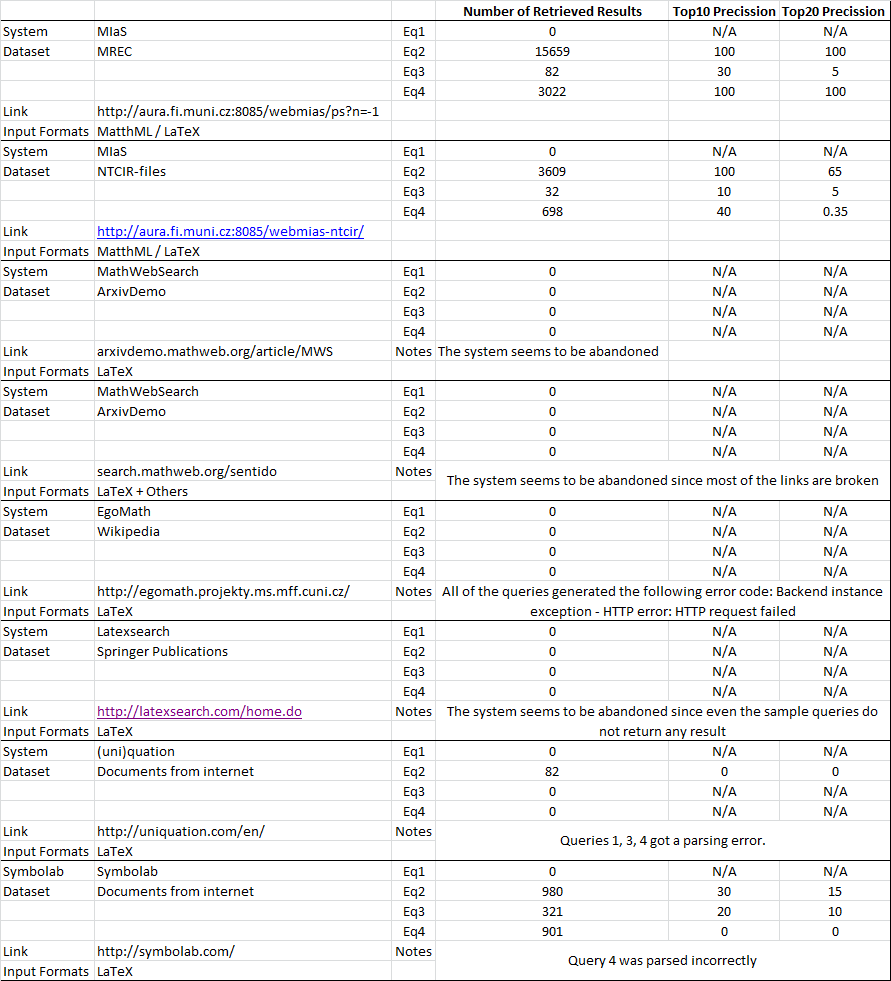
\includegraphics[height=15 cm]{figures/comparison_table.png}
\label{comparison_sw_table}
\caption{Results of comparison of available mathematical search systems}
\end{figure}

The results are a little disappointing since from the eight evaluated instances, only MIaS and Symbolab seem to be working properly. 

\section{Querying Performance}


\section{Indexing Performance}
For this set of evaluations, we were only interested in observing how the performance of the indexing stage is affected by the different types of features that are employed. We selected the first 100 records from our dataset and measured the total time it required to index all the elements in Solr using a python script and the solrpy library to do the communication. The default similarity in Solr was used. We also measured the index size at the end of each experiment.
Our four scenarios were organized as follows:
\begin{itemize}
\item N : Only notational features over the original expression were used
\item N+S : Notational and structural features over the original expression
\item N+S+NN : Notational and structural features over the original expression and notational features over the normalized string using Mathematica's Simplify function
\item N+S+FN : Notational and structural features over the original expression and notational features over the normalized string using Mathematica's Full Simplify function
\end{itemize}

Table \ref{indexing_performance} summarizes the results of this set of experiments. The first result is the significant increase in processing time when using Mathematica. Going from the N scenario to N+S represent an increase of almost 15x in the indexing time. Adding standard normalization increases the indexing time by a factor near to 1.44x and full normalization by a factor of 1.55x.

With respect to storage size, we see a small footprint (Less than 5\%)in the total size by going from N to N+S. Adding normalization represents an increase by a factor of 1.78x and the size of the fully normalized index represents a smaller increase (1.76x)

We can observe that there is a small trade-off between time and storage size depending on which normalization mode is employed.

\begin{longtable}{|c|c|p{2cm}|p{2cm}|p{2cm}|}
\hline 
Feature Set & Total time (sec) & Index Size (kb) & Avg. time per equation & Avg. size of equation (kb) \\ 
\hline 
N & 58 & 13926 & 0.00524 & 1.237 \\ 
\hline 
N+S & 884 & 14438 & 0.0785 & 1.282 \\ 
\hline 
N+S+NN & 1273 & 25780 & 0.113 & 2.345 \\ 
\hline 
N+S+FN & 1377 & 25548 & 0.122 & 2.269 \\ 
\hline
\caption{Indexing performance}
\label{indexing_performance}
\end{longtable} 


















\bibliographystyle{unsrt}
\addcontentsline{toc}{chapter}{Bibliographie}
\nocite{*}
\thispagestyle{empty}
\bibliography{bibliographie}
\begin{appendix}
\appendix
%\chapter{Annexes}
\label{app}


\section{Conception des masques}
\label{masque}



Le tableau \ref{masque} regoupe les dimensions du masque et les dimensions pr�vues .

\begin{table}[!ht]
\renewcommand{\arraystretch}{1}
\centering
\begin{tabular}{l r r }
\toprule
\textbf{}					&\multicolumn{2}{c}{\textbf{Dimensions}} \\ 
\textbf{Param�tres} 					& \textbf{sur masque}	& \textbf{sur wafer} \\
\midrule
Largeur des lames souples			& $3\mu m$ 				& $2.5\mu m$ 	\\
Largeur des lames rigides			& $2.5\mu m$ 			& $2  \mu m$ 	\\
Largeur d'une dent large			& $5 \mu m$				& $4.5 \mu m$	 \\
Largeur d'une dent �troite			& $4 \mu m$				& $3.5 \mu m$	 \\
Gap (rotor/stator)					& $1 \mu m$				& $1.5 \mu m$ 	 \\
\midrule
Largeur des lames du robot v 2.5	& $2.5\mu m$ 				& $2\mu m$ 	\\
Largeur des lames du robot v 2.0	& $2.0\mu m$ 				& $1.5\mu m$ 	\\
Largeur des lames du robot v 1.5	& $1.5\mu m$ 				& $1\mu m$ 	\\
Largeur des lames du robot v 1.0	& $1.0\mu m$ 				& $0.5\mu m$ 	\\
\bottomrule
\end{tabular}
\caption{Dimensions des param�tres sur le masque de la deuxi�me verison et dimensions pr�vues sur wafer}
\label{table:masque}
\end{table}

La fabrication et la mise au point du processus de fabrication a �t� donn� � une personne externe. Le lecteur est invit� � se r�f�rer aux annexes \ref{process flow} et \ref{runcard} pour le processus en lui-m�me.

\section{Constantes physiques et propri�t�s des mat�riaux}
\label{constantes}

Les valeures suivantes ont �t� utilis�es pour les applications num�riques. Afin de s'affranchir des propri�t�s anisotropes du silicium, les valeurs les plus contraignantes de ces propri�t�s ont �t� consid�r�s. Un coefficient de s�curit� de 10 a �t� pris pour les contraintes admissibles maximum.

\begin{table}[!ht]
\renewcommand{\arraystretch}{1}
\centering
\begin{tabular}{lcr@{}l}
\toprule
\textbf{Param�tres} 			& \textbf{Symboles}	& \multicolumn{2}{c}{\textbf{Valeurs}} \\
\midrule
Module de Young					& $E$				& $160$				& $GaOP$ \\
Contrainte admissible 			& $\sigma_{adm}$ 	& $7\times 10^8$ 			& $ Nm^-2$ \\
Permitivit� de l'air 			& $\epsilon$ 		& $8,85\times 10^-12$ 		& $C^2 N^-1m^-2$ \\
\bottomrule
\end{tabular}
\caption{Constantes physiques et propri�t�s des mat�riaux}
\end{table}

%http://fr.wikipedia.org/wiki/Th%C3%A9orie_des_poutres




\section{Contenu du CD-ROM}
\label{cd}


Le CD-ROM contient les fichiers suivants:

\begin{itemize}
\item $Latex$: Rapport du projet de semestre.
\item $Matlab$: Programme de traitement d'image pour mesure dynamique.
\item $Labview$: Programme de commande du micromoteur.
\item $process flow$: Processus de fabrication
\item $runcard$: Protocole du processus de fabrication.
\item $solidworks$: Conception assist�e par ordinateur du moteur.
\item $Cl�win$: Masques sous format .cif
\item $microscopie MEB$: Image prise par Microscopie Electronique � Balayage MEB.
\item $Excel$: Traitement des r�sultats.
\end{itemize}





\section{Processus de fabrication}
\label{process flow}





\section{Protocole du processus de fabrication}
\label{runcard}





\section{Article en cours d'impression: ``Three-Phase Electrostatic Rotary Stepper Micromotor with a Flexural Pivot Bearing''}
\label{annexe_confidential}




\section{Article de la conf�rence Transducers 2009: ``Single mask 3-phase electrostatic rotary stepper micromotor''}
\label{annexe_transducers}







\end{appendix}
\end{document}






